\section{Introduction}
In this chapter will be presented briefly the Kundera modular architecture, the way in which Kundera is supposed to be extended, the problems occurred in the process and how the community helped in achieving the result.
Then are discussed the detail of the two Kundera extension developed, in section \ref{sec:kundera-datastore} the one for Google Datastore and in section \ref{sec:kundera-table} the one for Azure Table.

\section{Overview of Kundera}
Kundera \cite{online:kundera} is an implementation of the JPA interface that now supports various NoSQL datastore. It supports by itself cross-datastore persistence in the sense that its allows an application to store and fetch data from different datastores.
Kundera provides all the code necessary to implement the JPA 2.1 standard interface independently from the underlying NoSQL database. 

\newparagraph The currently supported NoSQL databases are:
\begin{itemize}
\item Oracle NoSQL (versions 2.0.26 and 3.0.5)
\item HBase (version 0.96)
\item MongoDB (version 2.6.3)
\item Cassandra(versions 1.2.9 and 2.0.4)
\item Redis (version 2.8.5)
\item Neo4j (version 1.8.1)
\item CouchDB (version 1.0.4)
\item Elastic Search (version 1.4.2)
\end{itemize}

\begin{figure}[tbh]
  \centering
  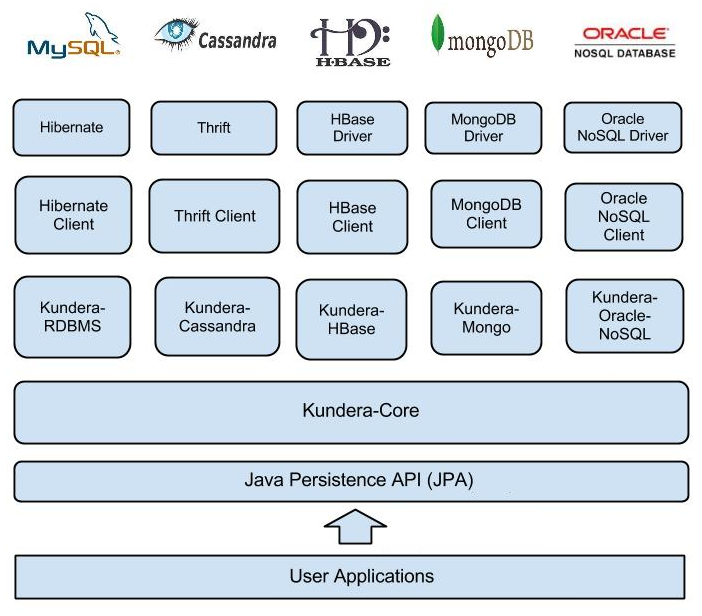
\includegraphics[scale=0.5]{images/kundera_architecture}
  \caption{Kundera architecture}
  \label{fig:kundera_architecture}
\end{figure}

\newparagraph The architecture of Kundera is shown in Figure \ref{fig:kundera_architecture}. The figure highlights the fact that the user application interacts with Kundera simply by exploiting the standard JPA interface implemented in the Kundera-Core.
Kundera-Core, each time an operation need to be executed on the underlying database, delegates the operation to the appropriate \texttt{Client} creating it through a \texttt{Client Factory} if it does not exists yet.

\subsection{Kundera's Client Extension Framework}
Kundera try to offer a common way to interacts with NoSQL databases through a well defined interface and as on open source project make other developers able, if interested, in using and extending it adding support to other datastore.
Is so available a Client Extension Framework descripted in the Kundera wiki which provides a short introduction on how Kunders clients should work and provides the interfaces and classes that should be developed in order to make the client work properly.

\newparagraph Basically to build a new Kundera client, these are the blocks to be developed:
\begin{itemize}
\item the \texttt{Client}, which is the gateway to CRUD operations on database, except for queries;
\item the \texttt{Client Factory}, which is used by Kundera to instantiate the Client;
\item the \texttt{Query implementor}, which is used by Kundera to run JPA queries by invoking appropriate methods in Entity Readers;
\item the \texttt{Entity Reader}, which is used by Kundera to translate the queries into correct client
method calls;
\item optionally the \texttt{Schema Manager}, to support automatic schema generation.
\end{itemize}

\subsection{Approaching the extension}
It all seems quite simple but the problem is that the documentation is actually outdated. 
Two were the main problem in understaing what to do and how, firstly it turns out that the required interfaces are actualy a little different and also are the required methods
secondary, and slightly more time consuming, is that no hints nor documentation are given on the structure and informations carried by the methods arguments.
The arguments carrys data structures containing informations organized in the kundera metamodel which is the implementation of the JPA metamodel that contains all the information associated (throug annotations) to a class or a field.

\newparagraph Due to those problems and to shrink the developing time, the solution was to write on the Kundera google group page to ask the community for more updated infos about Kundera extension.
Briefly an answer has come and I've started a conversation with one of the developers of Kundera who helped me giving the updated informations for the Kundera's Client Extension Framework and tell me to look forward to the other client implementation for some examples. 
Thanks to the updated information it turns out that the \texttt{Entity Reader} was unnecessary and all the translation from JPA queries to datastore specific queries and their executions should be done in the \texttt{Query Implementor}.  

\noindent At this point since no answer were given about the Kundera metamodel, the most valid solution was to approach the extesion as a test driven development, so, looking at the tests code of the other clients, I've writed a set of unit tests one for each feature.
With the tests failing and studyng the code of the other Kundera clients was then possible to reverse engineer the arguments thath were not documented and thus be able to develop the new extensions.

\newparagraph Unit tests are analyzed in detail in the chapter \ref{chap:eval}.

\section{Developing client extensions}
Have been developed two different extension for Kundera, the first one for Google Datastore and the second one for Azure Table.
After a first difficulty in figuring out how the extension have to be carried out, a main structure has been defined so the two projects have many parts in common. 
In the following sections the extensions are presented separately, the concepts are introduced as they are encountered and will be referenced further on if necessary specifying the differences if any.

\subsection{Google App Engine Datastore client}
\label{sec:kundera-datastore}
The first extension that has been faced is the one for Google App Engine (GAE) Datastore \cite{online:datastore} the NoSQL solution available in the App Engine runtime, is a key-value storage build on top of Google BigTable.

\subsubsection{JPA identifier}
In Google Datastore the most basic unit that can be stored is an Entity which is identified by a Key and composed of Properties.
Entities Keys contains various information about the entity itself:
\begin{itemize}
\item the entity Kind, which is used to group entities of the same type;
\item an entity identifier, used to distinguish entities of the same type;
\item an optional parent entity. 
\end{itemize}
Inspired by the Google JPA implementation on Datastore the idea was to use the Java class representing the datastore Key as indentifier for the POJO but unfortunately this was not possible since Kundera support only a pre defined set of Java datatypes.

\newparagraph The adopted solution is to handle the key internally, each time an opertion is required on Datastore the key relative to the entity is builded, the key Kind is directly mapped to the table name and the Key identifier is the user defined id in the \texttt{@Id} annotation.

\noindent IDs can be specified by the user or automatically generated, there are three possibilities:
\begin{itemize}
\item \texttt{@Id} annotation on a \texttt{String} type field
\item \texttt{@Id} annotation on a \texttt{Long} type field
\item \texttt{@Id} annotation on a primitive \texttt{long} type field
\end{itemize}
For each case the ID can be user specified before the persist operation but in case of ID auto-generated the field must be of type \texttt{String} and the generated ID will be a string representation of a random java \texttt{UUID}.

\noindent Auto-geenerated ID are supported by Kundera thorugh \texttt{@GeneratedValue} with \texttt{AUTO} or \texttt{TABLE} strategy, only \texttt{AUTO} strategy is supported. 
It was not possible to use the Datastore API to generate IDs since is necessary to know the Kind of the entity to be persisted but neither the \texttt{AUTO} strategy nor the \texttt{TABLE} one provides this infomation at generation time.

\subsubsection{Consistency}
In Datastore entities are organized in Entity Groups based on their Ancestor Path, the ancestor path is a hierarchy containing the keys of the entities which are parents of the given one and thus in the same entity group.

\noindent Consistency is managed through Entity Groups and so by defining the ancestor paths, entities within the same Entity Groups are managed in storng consistency, eventual consistency is used otherwise.

\noindent Datastore provide the possibility to create Ancestor path by defining entities parent to other entities and is basically a task left to the user, no automated sorting or guessing is provided. Other wrapper around Datastore low-level API also leave this to the user, for example in Objectify \cite{online:objectify} the developer make use of an \texttt{@Parent} annotation that make the user able to specify the Ancestor Path.
Since JPA is well defined and adding such annotation will break the standard the only alternative way is trying to automatic guess the ancestor path.

\newparagraph Relationsips are clearly a good point where found information for guessing if two entitiy kind can be hirearchically related, so for each type of relation must be defined what solution can be adopted.
\begin{itemize}
\item for \textbf{One to Many} and \textbf{One to One} relationships, since there's an owning side, the owning entity can be used as parent for every related entity. 
\item \textbf{Many to One} can be skipped since are the inverse of \textbf{One to Many} so such related entities should be already organized. 
\item for \textbf{Many to Many}, since the realtionship is handeled through a join table, it does not make sense to relate the entities involved.
\end{itemize}

\noindent Also if possible this guessing was not done in the extension for two main reasons:
\begin{enumerate}
\item entities are not require to have a single relationship
\item entities with a parent require the parent Key to be universally identified
\end{enumerate}
So for the first reason is impossible, unless asking to the user, to decide which relation use to hierarchically organize entities, furthermore for the second reason when declaring a entity parent to another is always necessary to know the Key of the parent (and thus its Kind and identified) beside the Key of the entity itself to be able to retrieve it from Datastore and for how Kundera is structured this information is not available during find operation in which Kundera provides only the table name, the identifier and the entity class.

\newparagraph For those reasons was not possible, without causing errors, to automatically guess ancestor paths through JPA relationships or make the user able manage them directly through a specific annotation.
Each Kind is persisted as a root Kind and so each entity is stored in a separated entity group identified by its Kind (the name of the JPA table associated to the entity).

\subsubsection{JPA relationships}
All the JPA supported relationships \cite{book:projpa2} has been implemented in the client and  have been implemented like they would be in a RDBMS system.
So for \textbf{One to One} and \textbf{One to Many} relationships on the owning side of the relationships a \textit{reference} to the non-owning side entity is saved.

\noindent For \textbf{Many to One} relationships there would be two solutions:
\begin{itemize}
\item persist a list of \textit{references} tp the related entities;
\item do not persist anything within the entity and fill the relationship with a query.
\end{itemize}
The second solution has been adopted since more consistent with other Kundera client implementation and with the classic implementation of this relation type in RDBMS.
\noindent For \textbf{Many to Many} relationships a join table is created based on user directives specified in the POJO annotations. The join table is filled each time a many to many related entity is persisted and a new \textit{row} is created inside the join table with the \textit{references} to the entities involved in the relationship.

\noindent The so far called \textit{reference} for Datastore is exploited by persisting within the entity the Key (Kind and identifier) of the related entity.

\subsubsection{Queries}
Queries in Kundera are supported in JPQL the JPA query language which is a  object oriented query language based on SQL \cite{book:projpa2}.
Kundera supports all of the clauses of JPQL but with some restrictions, clauses can be applied on:
\begin{itemize}
\item primary key attributes (\texttt{@Id}) and column attributes (\texttt{@Column}).
\item combination for primary key attribute and columns.
\end{itemize}

\newparagraph The JPQL query is parsed and validated by Kundera and to the \texttt{Query Implementor} is provided a filled metamodel of the query which needs to be \textit{explored} in order to build a datastore compatible query.    
Datastore have on its own a very good support to queries so all the clauses are supported except for the \textit{LIKE} operator.

\noindent In table \ref{table:queries} can be found a complete list of the supported JPQL clauses for both extensions.

\begin{table}[p]
\centering
\begin{tabular}{|l|c|c|}
\hline
\textbf{JPA-QL Clause} & \textbf{Datastore support} & \textbf{Table support}\\ 
\hline\hline
\textit{SELECT}        & yes 	& yes 	\\ \hline
\textit{UPDATE}        & yes 	& yes 	\\ \hline
\textit{DELETE}        & yes 	& yes 	\\ \hline
\textit{ORDER BY}      & yes 	& no 	\\ \hline
\textit{AND}           & yes 	& yes 	\\ \hline
\textit{OR}            & yes 	& yes 	\\ \hline
\textit{BETWEEN}       & yes 	& yes 	\\ \hline
\textit{LIKE}          & no  	& no  	\\ \hline
\textit{IN}            & yes  	& no  	\\ \hline
\textit{=}             & yes 	& yes 	\\ \hline
\textit{\textgreater}  & yes  	& yes 	\\ \hline
\textit{\textless}     & yes 	& yes 	\\ \hline
\textit{\textgreater=} & yes 	& yes 	\\ \hline
\textit{\textless=}    & yes  	& yes 	\\ \hline
\textit{Projections}   & yes  	& yes 	\\ \hline
\end{tabular}
\caption{JPQL clauses support for the developed extension}
\label{table:queries}
\end{table}

\subsubsection{Embedded entities}
Embedded fields are supported by the JPA \cite{book:projpa2} annotating the field that needs to be embedded with the \texttt{@Embedded} annotation and annotating the corresponding POJO with the \texttt{@Embeddable} annotation.

\newparagraph Implementation of those kind of entities is straightforward for Datastore because it supports tehm natively as Embedded Entity.
\noindent The implementation so make use of this feature translating the embeddable POJO in a Datastore embedded entity and then persist it within the parent entity.

\subsubsection{Collection fields}
JPA standard supports collection or maps to be used as entities field throug the annotation \texttt{@ElementCollection}.

\newparagraph Lists are natively supported by Datastore but are supported only if composed of primitives Java datatypes.
\noindent To be able to save whatever kind of collection or map independently by the datatype thath compose it, the collection or map itself is serialized to a \texttt{byte} array when persisted and deserialized when readed.
\noindent To simplify the developing, also Lists of primitive types, even if supported natively, are serialized.

\subsubsection{Enum fields}
Enum fields are supported by the JPA through the annotation \texttt{@Enumerated}  simply by persisting its string represention and instantiating the corresponding enum type back when the entity is read.

\subsubsection{Schema Manager}
Schema manager as required by Kundera has to exploit four operations:
\begin{itemize}
\item \textit{validate}, which validates the persisted schema based on entity definition.
\item \textit{update}, which updates the persisted schema based on entity definition.
\item \textit{create}, which create the schema and thus the tables based on entity definitions.
\item \textit{create\textunderscore drop}, which drops (if exists) the schema and then re-creates it by re-creating the tables based on entity definitions.
\end{itemize}

\noindent The first two cases are quite useless for a Datastore since there's no fixed schema for entities, entities with same Kind can have different Properties withouth restriction.
Also the \textit{create} case is usless for Datastore since if a new entity of an unknown Kind is persisted it's created without the need to explicitly define it first as a new Kind.
The last case \textit{"create\textunderscore drop} will so just drop the current schema, deleting all the persisted Kind(s) and so all the related entities, without re-creating the schema since it constructs by itself.

\subsubsection{Datastore specific properties}
Kundera offers the possibility to define some datastore specific properties in an external xml file that need to follow a simple structure. This file is referenced inside the \texttt{persistence.xml} and is optional.

\newparagraph This possibility is exploited by the Datastore extension and make the user able to configure the following properties:
\begin{itemize}
\item \texttt{datastore.policy.read}, to set the read policy
\item \texttt{datastore.deadline}, to define the RPCs calls deadline
\item \texttt{datastore.policy.transaction}, to specify if Datastore have to issue implicit transactions
\end{itemize}
Those properties are read in the \texttt{Client Factory} and used to initialize the datastore connection with the required parameters.

\newparagraph For a complete reference for Google Datastre extension configuration see the appendix \ref{appendix:datastore-config}.

\subsection{Azure Table client}
\label{sec:kundera-table}
Azure Table \cite{online:azuretable} is the NoSQL solution developed by Microsoft, is a key-value storage and it's available inside Azure environment.

\subsubsection{JPA identifier}
In AzureTable an entity to be persisted must either implement a special interface \texttt{TableServiceEntity} or be translated into a \texttt{DynamicEntity} which is basically a property container.
An entity is then uniquely identified inside a table by a \texttt{partitionKey} and a \texttt{rowKey}.
\noindent Partition keys are used to handle consistency, strong consistency is guaranteed while entities are stored within the same partition key otherwise consistency will be eventual.

Since both partition key and row key are are supported only in field of type \texttt{String} and since the JPA annotation \texttt{@Id} can be declared on only one field per POJO, partition key adn row key are concatenated in a single \texttt{String} and hadled internally by the extension through the class \texttt{AzureTableKey} builded ad hoc since for Table ther's no a class similar to \texttt{Key} of Datastore.
\noindent This way the user have complete control over partition key and row key and thus on the consistency mechanism.

\newparagraph Are available for the user three different approaches to handle those identifiers:
\begin{enumerate}
\item define manually both row key and partition key
\item define manually only the row key 
\item let the extension to completely handle the identifier annotating the ID field also with \texttt{@GeneratedValue(strategy = GenerationType.AUTO)}
\end{enumerate}

\noindent For the first case, to help the user in defining both the partition key and the row key indipendently of the way the extension handle them, a static method \texttt{AzureTableKey.asString(String partitionKey, String rowKey)} is provided. Is not required its usage but in this case the ID must follow the convention used by the extension which is \texttt{partitionKey\textunderscore rowKey}.
\noindent The second case is exploited setting the ID to a string value, this value is interpreted by the extension as the row key while the partition key is set to a default value that can be modified in the datastore specific property file described later on. Also for this case, to have a more fluent API an utility method is provided: \texttt{AzureTableKey.asString(String rowKey)} 
\noindent The third and last method will generate a java random \texttt{UUID} for the row key and set the partition key to the default value.

\subsubsection{JPA relationships}
Also for Azure Table relationships are implemented similary to RDBMS as described previously for Datastore (\ref{sec:kundera-datastore}).

\noindent The only difference is that when is needed to keep a \textit{reference} to another entity, is persisted within the entity the partition key and the row key of the related entity.
Even if the pair partition key and row key is not sufficient to identify an entity universally, it is sufficient for Kundera since the information of the table is available to the client just by looking at the metadata of the relationship. 

\subsubsection{Queries}
Supporting queries for Azure Tables was straightforward, the procedure was the same described in \ref{sec:kundera-datastore} but due to the different operator supported by Tables, beside the \textit{LIKE} operator also the \textit{IN} operator is not supported.

\noindent In table \ref{table:queries} can be found a complete list of the supported JPQL clauses for both extensions.

\subsubsection{Embedded entities}
Embedded fields (described in \ref{sec:kundera-datastore}) are not supported natively by Azure Table so the solution adopted is to serialize the field annotated with \texttt{@Embedded} to be able to persist it to the storage like a \texttt{byte} array and deserializing it when the entity is read.

\subsubsection{Collection fields}
As described for Datastore (\ref{sec:kundera-datastore}) JPA supports collections but are not supported in Azure Tables even if composed of the supported datatypes.

\noindent To support even complex collection or maps the obvious solution is to serialize the entire collection or map to a \texttt{byte} array when persisting the entity and deserialize it when reading the entity from the storage.

\subsubsection{Enum fields}
Enum fields are supported by the JPA through the annotation \texttt{@Enumerated}  simply by persisting its string represention and instantiating the corresponding enum type back when the entity is read.

\subsubsection{Schema Manager}
Schema manager (as described in \ref{sec:kundera-datastore}) have been also implemented for Azure Table and like Google Datastore, the first two cases are quite useless since ther'se no fixed schema and entities within the same Table can have different properties withouth restriction.

\newparagraph Azure Table need that the Table in which entities are stored exists before trying to create entities so the \textit{create} case simply iterate over all table names and creates it in the database. 
For the \textit{create\textunderscore drop} case, all tables should be dropped (and so all the contained entities) and re-created. The problem here is that Tables deletion is performed asynchronously and so exists an unpredictable amount of time in which the table cannot be re-created since it still exists even if not listed.
\noindent To overcome to this problem two solution can be adopted:
\begin{itemize}
\item catch the \texttt{StorageException} thrown when the table is creaed while still exists, put the process to sleep for an amount of time and try again
\item do not delete the Table itself but delete all its entities in bulk
\end{itemize}

\noindent The first method is clearly dangerous since no deadline is given for the Table delete operation, the second solution is actually not so convenient because, even if deletion is performed as a batch operation both the partition key and row key must be specified and thus a query must be performed over the table to retrieve at least partion key and row key for each entity in the table.  

\noindent So for the \textit{create\textunderscore drop} case is performed a drop of all the Tables and then are re-created even if this can cause the previously mentioned conflict, this option is left as is for testing purposes since in the storage emulator the problem is not showing because the Table storage is emulated over a SQL server instance.

\subsubsection{Datastore specific properties}
As described for Datastore (\ref{sec:kundera-datastore}), Kundera provides a datastore specific properties file that let the user set some specific configuration.

\noindent This possibility is supported also for Azure Tables with the following properties:
\begin{itemize}
\item \texttt{table.emulator} and \texttt{table.emulator.proxy}, to make the user able to test against the local storage emulator on Windows
\item \texttt{table.protocol}, to make the user able to decide between \textit{http} or \textit{https} for storage calls
\item \texttt{table.partition.default}, to let the user specify the value for the default partition key 
\end{itemize} 

\newparagraph For a complete reference for Azure Table extension configuration see the appendix \ref{appendix:table-config}.

\section{Summary}
In this chpater has been introduced in details how Kundera extension should been developed, the problem encountered during the development, how tey've been addressed and the detail of the implementation of the two extensions including the feature that are currently supported.
In the next chapter will be explained how has been possible to integrate Kundera into CPIM as part of the NoSQL service.
